\documentclass{article}
\author{Trever Hallock}
\title{Final Project}

\usepackage{listings}
\usepackage{amsmath}
\usepackage{graphicx}

\begin{document}

\maketitle

\pagebreak

\section{Introduction}
Shortest path problems are frequently encountered within optimization, as many problems can be modeled with a graph in which a solution is a path between two nodes of the graph.
For example, we can interpret nodes to be locations, arcs to be roads between these locations, and assign the weights to be travel times along these edges.
In this case, the fastest travel time between two locations is a shortest path problem.
Shortest path problems play an important role in column generation for linear programs and shortest path routines can be used within other algorithms, such as the generic path augmenting algorithm for maximum flow problems.
Shortest path problems are nice in the sense that they are tractable: Dijkstra's algorithm finds a shortest path through $G=(V,E)$ within $O(|V|^2)$ time 
(or $O(|E| + |V| \log |V|)$ with an efficient min-priority queue).

However, I was not able to find many attempts to parallelize the search for a shortest path.
After much searching, I did find \cite{par1}, \cite{par2} and \cite{par3}.
One approach for parallelization is allow multiple threads to remove nodes from the horizon, or set of marked nodes, in parallel.
This allows the efficiency to scale with the width of the graph, but introduces complications when nodes removed at the same time by different threads are both incident with an edge of the shortest path.

In this paper, I describe a new parallel algorithm that uses two processors to improve the running time.
One thread is assigned to the source node, and another to the destination node.
Then each runs Dijkstra's algorithm torward the other until they ``meet."

We will begin with a description of the algorithm and prove its correctness.
Then we will discuss the running time of this version compared to a single threaded version of Dijsktra before making closing remarks.

\section{The Algorithm}

\subsection{Notation}
Let $G = \{E, V\}$ be a graph, where $V = \{i\in Z| 1\le i \le n\}$ and each edge $(i,j) \in E \subseteq V \times V$ has associated cost $c_{ij} \ge 0$.
We are concerned with finding an $s-t$ path in $G$ with least cost.
We define the intersection of a path with a set $K\subseteq V$ to be the intersection of the set of all nodes in the path with set $K$ of nodes.
Also, we define the concatenation of paths $S=(s_1, s_2, \ldots, s_{|S|})$ and $T=(t_1=s_{|S|}, t_2, \ldots, t_{|T|})$
to be the path $(S,T) = (s_1, s_2, \ldots, s_{|S|} = t_1, t_2, \ldots, t_{|T|})$.

Note that in the following description, a
\begin{lstlisting}
#BARRIER n
\end{lstlisting}
denotes a barrier that all threads must reach before proceeding.

Also, $tnum \in \{1,2\}$ is a thread-local variable representing the thread id of the thread executing.
For convenience, we will let 
\[
 other(i) =
  \begin{cases} 
      2 \hfill \quad i = 1 \\
      1 \hfill \quad i = 2 \\
  \end{cases}
\]

\subsection{Pseudo-code}

If we run Dijkstra's algorithm from both the source node and sink node, we will have the following pseudo-code, up until barrier 1.
After that, we patch together something akin to an $[S,T]$ cut formed between the nodes labeled by the two threads.
The two threads ``meet" when a thread discovers that it has labeled a node already labeled by the other thread.
This is a cut except for the 1 (or sometimes 2) nodes that end up being labeled by both threads.
At this time, the two threads iterate over their respective heaps looking for possible edges between the two sets of labeled vertices.


\begin{lstlisting}

	
	
	Lock MinPathSync
	MinPath = ()
	MinPathCost = infty
	
	FoundByOneThread = false

	beginNode(1) = s;
	beginNode(2) = t;
	endNode(1) = t;
	endNode(2) = s;
	
	stopSearch = false
	
	#BEGIN PARALLEL
	
	for all v in V - beginNode(tnum)
		dist(v, tnum) = infty
	dist(beginNode(tnum), tnum) = 0
	marked(beginNode(tnum), tnum) = true
	Heap[tnum] = {beginNode(tnum)}
	intersection[tnum] = -1
	
	
	# BARRIER 0
	
b1	while  Size(heap[tnum]) > 0
		if stop
b2			break
		endif
		
r1		v = RemoveSmallest (heap[tnum])
u1		marked(v, tnum) = false
l1		labeled(v, tnum) = true
		
f1		for all (v,u) in (tnum == 0 ? E : Reverse(E))
m1			marked(u, tnum) = true
g1			if dist(v, tnum) + cost((v,u)) <
					dist(u, tnum)
d1				dist(u, tnum) = dist(v, tnum) 
					+ cost((v,u))
p1				Prev(u, tnum) = v
a1				AddOrUpdateKey(heap[tnum], u)
			endif
		endfor
		
		if labeled(v, other(tnum))
			stop = true
			intersection[tnum] = v
b3			break
		endif
		
		if v == endNode[tnum]
			// This thread found the whole path.
e1			FoundByOneThread = true
		endif
	endwhile
	
	if not stop
		// The source is not connected to the destination
		return NULL
	endif
	
s1	#BARRIER 1
	if FoundByOneThread
l1		return Optimal path found by a single thread.
	endif
	
	if intersection[tnum] >= 0
c1		P = Concatenate(
			GetPath(intersection[tnum],tnum), 
			GetPath(intersection[tnum], other(tnum)))
		Lock(MinPathSync)
		if Cost(P) < MinPathCost
			MinPath = P
			MinPathCost = Cost(P)
		endif
		Unlock(MinPathSync)
	endif
	
	for u in Heap[tnum]
		if Labelled(u, other(tnum))
			v = Prev(u, tnum)
			P = Concatenate(GetPath(v,tnum),
					((u,v)),
					GetPath(u, other(tnum)))
			Lock(MinPathSync)
			if Cost(P) < MinPathCost
				MinPath = P
				MinPathCost = Cost(P)
			endif
			Unlock(MinPathSync)
		endif
	endfor
	
	#BARRIER 2
	
	return MinPath
\end{lstlisting}

%			// The other thread will either not start 
%			// 	or find its beginNode is already labeled.
%			// Set a flag to simply return the path from only this thread.
%			// Parallelizing this was pointless for this graph

\section{Proof of correctness}

Our proof will be a modification of \cite{dijk}.
It will proceed with induction on the set of labeled nodes.
This set is always increasing, as there is no assignment of the form 
\begin{lstlisting}
labeled(v, tnum) = false.
\end{lstlisting}

\subsection{Dijkstra's Algorithm before barrier 1}

Suppose that the parallel Dijkstra algorithm has been running for some time.
Let $L_i$ is the set of all vertices labeled by thread $i$.
We let $U = V - (L_1 \cup L_2)$ be the set of all unlabeled vertices. 
We can let $M_i$ be the set of all vertices that have been marked by thread $i$ and not labeled-that is, the nodes contained into Dijsktra's heap.
By definition,
$$M_1 \cap L_1 = M_2 \cap L_2 = \emptyset$$
as vertices that leave the heap in r1 are immediately labeled in line l1.

%$$U = V - ((\cup_{i\in \{1,2\}} L_i) \cup (\cup_{i\in \{1,2\}} M_j))$$ 

We can let $d_s(v)$ be the distance from $s$ to node $v$, and $d_t(v)$ be the distance from node $t$.
By optimality conditions, these satisfy $d_s(v) \le d_s(u) + c_{uv}$ and $d_t(v) \le d_t(u) + c_{uv}$
for all $(u,v) \in E$, as well as the existence of a path with cost $d_s(v)$ from $s$ to $v$ for all $v \in V$ if $d_s(v) < \infty$ (and likewise for thread 2).
%By stopping condition's assumption, we can let $w \in L_1 \cap L_2$, and 
%without loss of generality assume that
%the thread who labeled a vertex already labeled is thread 1.
%That is, $d_s(w) \ge d_s(v) \forall v \in L_1$ because the algorithm terminates \emph{immediately} after one thread finds a node already labeled by the other thread.

The first property we wish to show is that
$$\forall (u,v) \in E \quad u \in L_1 \Rightarrow v \in L_1 \cup M_1 $$
\begin{equation}
\forall   (u,v) \in E \quad u \in L_2 \Rightarrow v \in L_2 \cup M_2.
\label{eq:whereTheyAre}
\end{equation}
For any $i\in V$, we can define $Adj(i) = \{ j \in V | (i,j) \in E \}$.
Then \ref{eq:whereTheyAre} is true because immediately after a node $v$ is labeled in l1, all nodes in $Adj(v)$ are marked if not already marked in m1.
There is no way to leave the loop without having this happen.
Then, the only way nodes are unmarked is immediately preceding when they are labeled in u1.
This implies that $(L_1, V-L_1)$ is a cut with $\{ j \in V-L_1 | \exists i \in L_1, j \in Adj(i) \} = M_1$, and similarly for $M_2$.


The set $L_1$ only increases, as nodes are never unlabeled, so we proceed with two separate inductions on $L_1$ and $L_2$ until line b1, b2 or b3 is hit.
The induction hypothesis are the following:

$$dist(u,1) = d_s(u) \forall u \in L_1$$
\begin{equation}
dist(u,2) = d_s(u) \forall u \in L_2
\label{eq:equality}
\end{equation}
$$\exists s-u \quad \text{path} \quad P \subseteq L_1 \quad \text{with}\quad  C(P) = dist(u, 1) \forall u \in L_1 \cup M_1 $$
$$\exists u-t \quad \text{path} \quad P \subseteq L_2 \quad \text{with}\quad  C(P) = dist(u, 2) \forall u \in L_2 \cup M_2 $$
$$d_s(v,1) \le d_s(u,1) \forall v \in L_1, u \in V-L_1$$
\begin{equation}
d_t(v,2) \le d_t(u,2) \forall v \in L_2, u \in V-L_2
\label{eq:inOrder}
\end{equation}
$$dist(v,1) + c_{vu} \ge dist(u,1) \forall (v,u) \in L_1 \times M_1 \cap E$$
$$dist(v,2) + c_{vu} \ge dist(u,2) \forall (v,u) \in L_2 \times M_2 \cap E$$

%All nodes added to Heap[1] are in $M_1$.

%All nodes added to Heap[2] are in $M_2$.

%No node from $L_1$ is entered into Heap[1].

%No node from $L_2$ is entered into Heap[2].


This is clearly the case at line f1 of the first iteration, as $L_1 = \{s\}$ and $dist(u,1) = 0$ while $dist(u,1) = \infty$ for all $u \in V - L_1$.
The same holds for thread 2.
Now assume that the conditions are satisfied for several iterations.

First, we will show the first two properties.
Suppose that $v$ is the next smallest node removed by thread 1, and $d_s(v) < dist(v,1)$ so that there is an $s-t$ path $Q$ with cost $cost(Q) < dist(v,1)$.
Let $xy$ be the first edge of $Q$ leaving $L_1$, and $Q_x$ but the $s-x$ path in $Q$, so that $cost(Q_x) + c_{xy} \le cost(Q)$.
Also, by induction, we know that $dist(x, 1) = d_s(x) \le cost(Q_x)$ so $dist(x, 1) + c_{xy} \le cost(Q)$.
By definition, $v$ was in $M_1$. (Or just note that the way to be added to the heap is in line a1, immediately after m1.)
Thus, through induction, we find that $dist(y, 1) \le dist(x, 1) + c_{xy}$, because by equation \ref{eq:whereTheyAre}, $y \in M_1$.
Finally, because $v$ has the smallest $dist(v, 1)$, we know that $dist(v,1) \le dist(y, 1)$.
Altogether, we find $dist(v,1) \le dist(y,1) \le dist(x,1) + c_{xy} \le cost(Q) < dist(v,1)$ which is a contradiction.
This implies that $dist(v,1) = d_s(v)$, and there is an $s-v$ path of cost $dist(v,1)$.
A similar argument works for thread 2.
Because $v$ is the only node which is labeled in this iteration, the first and second hypothesis are true for this iteration.

Secondly, we with to show third and fourth properties.
The only way that a node $u$ is added to heap or has $dist(u,1)$ decreases is in line a1.
The only way to reach this line is by finding an edge from $v$ to $u$, and $v$ already has a path $P_v$ from $s$ with cost $dist(v,1)$.
Thus, $(P_v, u)$ is a path from $s-u$ with cost $dist(v,1) + c_{vu}$.
Note that this path is remembered with line p1.

The seventh and eighth properties follow from similar logic.
The induction hypothesis guarantees the identity for all but the newly added vertex (decreasing $dist(u,1)$ does not hurt this identity).
The new assignment is guarded with g1, and ensures that the identity is true for $v$ in addition to the vertices already in $L_1$.


For the fifth and sixth hypothesis, note that in d1, a node $u$ not yet labeled is decreased only to a positive number plus the cost of $v$ which was just added to $L_1$.
Because of the induction hypothesis, $dist(v,1) \ge dist(u,1) \forall u \in L_1$, so that $dist(u,1) \ge dist(v,1) \ge dist(u,1) \forall u \in L_1$.
Because they start at $\infty$, the induction hypothesis must remain true.
These were not explicitly used in the induction, but will be useful later.

Thus, the induction hypotheses are met for the next iteration, and continue to be true until the while loop is broken out of.
What happens then becomes the topic of the next section.


%One last observation is the following:
%Suppose this is not true, which necessarily implies $d_t(u, 1) < \infty$.
%Then If we ran dijsktra's algorithm for long enough we would add $u$ to the heap with $d_s(u) < d_s(v)$ when $v \in L_1$.
%However, the only way that $dist(u,1)$ decreases from infinity is 
%However, because the update of $dist(u, 1)$ in line d1 is the only such update, and it is guarded with a check that the new cost is less than its current cost, $dist(u,1)$ can only decrease
%(It actually can't, because it is already labeled.)
% Furthermore, at line f1 of the first iteration, nodes in $V-L_1$ have cost $\infty$, while the only node in $L_1$ has cost $0$.
% Assume that at line f1 after several iterations, we still have $dist(v, 1) \le dist(u, 1) \forall v \in L_1, u \in V-L_1$.
% Then a node $u$ in $V-L_1$ only has $dist(u, 1)$ decreased to be the $dist(v,1) + c_{vu}$ where $v \in L_1$ and $c_{vu} \ge 0$.
% Thus, at the end of this iteration , and similarly for $dist(v,2)$.
% 
% Node $u$ is only added to the queue in line a1,
% 
% which can only be reached $dist(u,1) >  in Because of this, if an edge from $u \in V-L_1$ to $v \in L_1$ is ever discovered, we
% 
% 
% 
% 
% 
% 
% 
% We want to show that $dist(v,1) \ge d_s(v) \forall v \in V$, and $dist(v,1) = d_s(v) \forall v \in L_1$.
% In order to show this, we need to show that for any $v$, there is a path with cost $dist(v,1)$,
% and when $v$ is labeled, $v$ satisfies $dist(v,1) \le d_s(u, 1) + c_{uv}$ for all other $u$.
% 
% 
% 
% First note that a node that has been removed from the queue can never reenter.
% A node $u$ is only entered in line a1 with the positive cost of an edge from a node $v$ that has been removed plus the cost of that node.
% This implies that for all $u \in V - 
% 
% 
% First node that $Prev(u,1) = v$ is executed in line p1 only if there is an edge from a node in $L_1$ to $u$.
% 
% 
% 
% 
% 
% %First, note that all nodes 
% This is clearly true during the first iteration, as $dist(v,1) = \infty$ for all $v\ne s$ while $dist(s, 1) = 0$.
% Suppose it is true at the beginning of an arbitrary iteration.
% From this assumption, we can conclude that the next node $v$ to be removed must already have $dist(v, 1) = d_s(v)$.
% 
% This is the case because all paths
% Then we have that $dist(u, 1)$ in d1 is only updated to be the cost of a node $v \in L_1$ plus the cost of an edge from $v$ to $u$.
% 

% 
% 
% Next we show that
% $$d_s(v) \le d_s(u) \quad \forall v \in L_1, u \in U$$
% \begin{equation}
%   d_t(v) \le d_t(u) \quad \forall v \in L_2, u \in U
% \label{eq:notAllNodeAreCreatedEqual}
% \end{equation}
% 
% This is clearly true for $L_1$ when $L_1 = \{beginNode\}$, as we have $dist(s)=0$.
% Next, assume that this is true for thread 1, at the beginning of an iteration through the loop.
% We know that 
% 
% 
% 


\subsection{Parallel Dijkstra}


The only way to exit the first while loop is to have $Size(Heap[tnum]) = 0$ or have stop be true in lines b1, b2 or b3.
If $Size(Heap[tnum]) = 0$, then the destination is not reachable from the source, as either $L_{tnum}$ is a cut with no edges going out (otherwise they would be in the heap!).
On the other hand, there are only two ways that stop = true.
The first is that one thread has found the entire shortest path at e1 so that this algorithm reduces to Dijkstra's algorithm when we leave at l1.
The second is that one thread discovers that a node just labeled has already labeled by the other thread in b2.
In this case, we have $L_1 \cap L_2 \ne \emptyset$, so that by the time s1 is executed, we can let $w \in L_1 \cap L_2$ (which is $intersection[tnum]$ for atleast one $tnum \in \{0,1\}$).

We note that if one thread finds the whole path, then we have just ran Dijkstra's algorithm, and have no need progress past the second barrier.
In this case, we can simply return the path found by one of the threads in l1.
Otherwise, by the time we reach Barrier 1 we know that 
$$ L_1 \ne \emptyset \ne L_2.$$

%From the results of the first section Dijkstra in \ref{eq:inOrder}, we have the following properties when we reach barrier 1:
%$$d_s(w) \ge d_s(v) \quad \forall v \in L_1 $$
%$$d_t(w) \ge d_t(v) \quad \forall v \in M_2.$$

Now consider a minimal path $P = (s = v_0, v_1, v_2, \ldots, v_{k_p-1}, v_{k_p} = t)$.
Also, let $P_s = (s = s_0, s_1, s_2, \ldots, s_{k_s-1}, s_{k_s} = w)$ and
$P_t = (w = t_0, t_1, t_2, \ldots, t_{k_t-1}, s_{k_t} = t)$ be the shortest paths found by the two Dijkstra's algorithms.
That is, $C(P_s) = d_s(w)$, $C(P_t) = d_t(w)$, and $P_s \subseteq L_1$, and $P_t \subseteq L_2$.
Our algorithm enumerates all edges from $M_1$ to $L_2$ and $L_1$ to $M_2$ in addition to the paths through each $w \in L_1 \cap L_2$.
Thus, in order to show correctness, we must show that there is an optimal path that satisfies these conditions.


\subsubsection{}
We have without loss of generality, 
\begin{equation}
P \cap U = \emptyset.
\label{eq:nullintersect}
\end{equation}
Specifically, we will show that if $P \cap U \ne \emptyset$, then $(P_s, P_t)$ is also a minimal path.
Because $(P_s, P_t) \subseteq L_1 \cup L_2$, so that $(P_s, P_t) \cap U = \emptyset$, we can just let $P=(P_s, P_t)$ in this case.
To this end, suppose that $$v_{u_1},v_{u_1+1},\ldots,v_{u_2-1},v_{u_2} \in P \cap U$$
is a subpath of $P$. (It is fine for $u_1=u_2$, as a sum $\sum_{i}^{i-1} a_i := 0$.)

First, we note that $v_{u_1} \in U \Rightarrow d_s(v_{u_1}) \ge d_s(w)$ and $v_{u_2} \in U \Rightarrow d_t(v_{u_2}) \ge d_t(w)$ by \ref{eq:inOrder}.
Also, $\sum_{i=1}^{u_1} c_{v_{i-1},v_i} \ge d_s(v_{u_1})$ because otherwise we could replace $(v_0, v_1, \ldots, v_{u_1})$
with a shorter path to find an $s-t$ path shorter than $P$.
Similarly, $\sum_{i=u_2}^{k_p} c_{v_{i-1},i} \ge d_t(v_{u_2})$, so that
$$C(P) = \sum_{i=1}^{k_p} c_{v_{i-1},v_i} $$
$$ = \sum_{i=1}^{u_1} c_{v_{i-1},v_i} + \sum_{i=u_1+1}^{{u_2}-1} c_{v_{i-1},v_i} + \sum_{i=u_2}^{k_p} c_{v_{i-1},v_i} $$
$$ = d_s(v_{u_1}) + \sum_{i=u_1+1}^{{u_2}-1} c_{v_{i-1},v_i} + d_t(v_{u_2})$$
$$ \ge d_s(w) + 0 + d_t(w) = C( (P_s, P_t) )$$
so that we can simply let $P = (P_s, P_t)$ to obtain a path just as short that does not include nodes of $U$.

\subsubsection{}
Now, suppose that $P$ contains an edge $(l_1,l_2)$ from $L_1$ to $L_2$, without using node $w$.
If $l_1 \in L_2$ or $l_2 \in L_1$, then one of these nodes are in $L_1 \cap L_2$, and both such nodes are tested to be optimal on line c1.
Otherwise, $l_1 \not \in L_2$ and $l_2 \not \in L_1$ and by \ref{eq:whereTheyAre} we know $(l_1, l_2) \in M_2 \times M_1$.
Between barrier 1 and barrier 2, the threads enumerate all edges from $M_1$ to $L_2$ and $M_2$ to $L_1$, including the path $(P_s, P_t)$.
We have just shown that $P$ contains no vertices but those in $L_1 \cup L_2$, and that if $P$ does not contain a node in $L_1 \cap L_2$,
then it contains an edge with a vertex in either $M_1$ or $M_2$.

(Another way to see this last property is to suppose that $\exists v_i : v_i \in P \cap M_1$.
If $v_i$ were not labeled by Thread $2$, then $v_i \in M_1 \Rightarrow v_i \not \in L_1$ and $v_i \not \in L_2$
together imply that $v_i \in U$, which cannot happen by \ref{eq:nullintersect}.
This is why we only need to consider the nodes within $M_1$ that are labeled by the other thread.)

\section{Comparison}
\subsection{}
My version of the single thread Dijkstra was not the best it could be, in the following sense.
In order to support searching backwards through the graph, I also had to maintain reverse edges.
This means that the graph had to be almost twice as large in memory, as as these graphs take a large amount of space, this could be a performance hit.

Another key observation is that we do not expect this to only improve times by a factor of $2$.
This is because the size of the horizon grows quickly (super-linearly) as a function of the distance from $s$ for dense graphs.
Thus, we would expect the horizon to be much larger at a distance $d_s(t)$ for a single threaded Dijkstra
than roughly the sum of two horizons at distance $\frac{d_s(t)} 2$.

I tested my algorithm on the following graphs.
One graph I tested on was the graph given on Canvas.
One type of graph was a randomly added graph with costs following a uniform distribution, and the probability $p$ of there being an edge between $(i,j) \in V \times V$
was uniform.
The second type of graph was a long graph with four different parameters: $w$ representing the width, $l$ representing the length, $r$ representing the look-back and $d$ representing the density.
This graph was created in the following way.
First $w$ disjoint paths of length $l$ were created.
To describe the rest, let me call each of the $l$ different sets of $w$ vertices of length $i$ (not cost) from $s$ ``stage $i$".
Then for for each of the $d$ stages, edges were randomly added to stage $i$ from any stage $j$ where $i-r \le j < i$ and $j \ge 1$.
The number of edges added was $d$ times the number of possible edges (which is $rw^2 - w$ because we have take away the edges from stage $i-1$ to $i$ that are already present).
Finally, I also ran my code on a complete graph.

%For example, if $r=l$ and $d=1$, then all 

\subsection{}
The results are summarized below.


For your graph, I ran all searches from node $53481$, and ran 21 separate $s-t$ path searches to each of the following vertices.
I recorded the time and speed up of parallelization for each. For all but one path, the speed up was greater than 1.
The average speed up was 2.99, while the speed of the average was 1.40.
I would conclude that for the types of graphs that these graphs came from, parallel Dijsktra is a good idea.

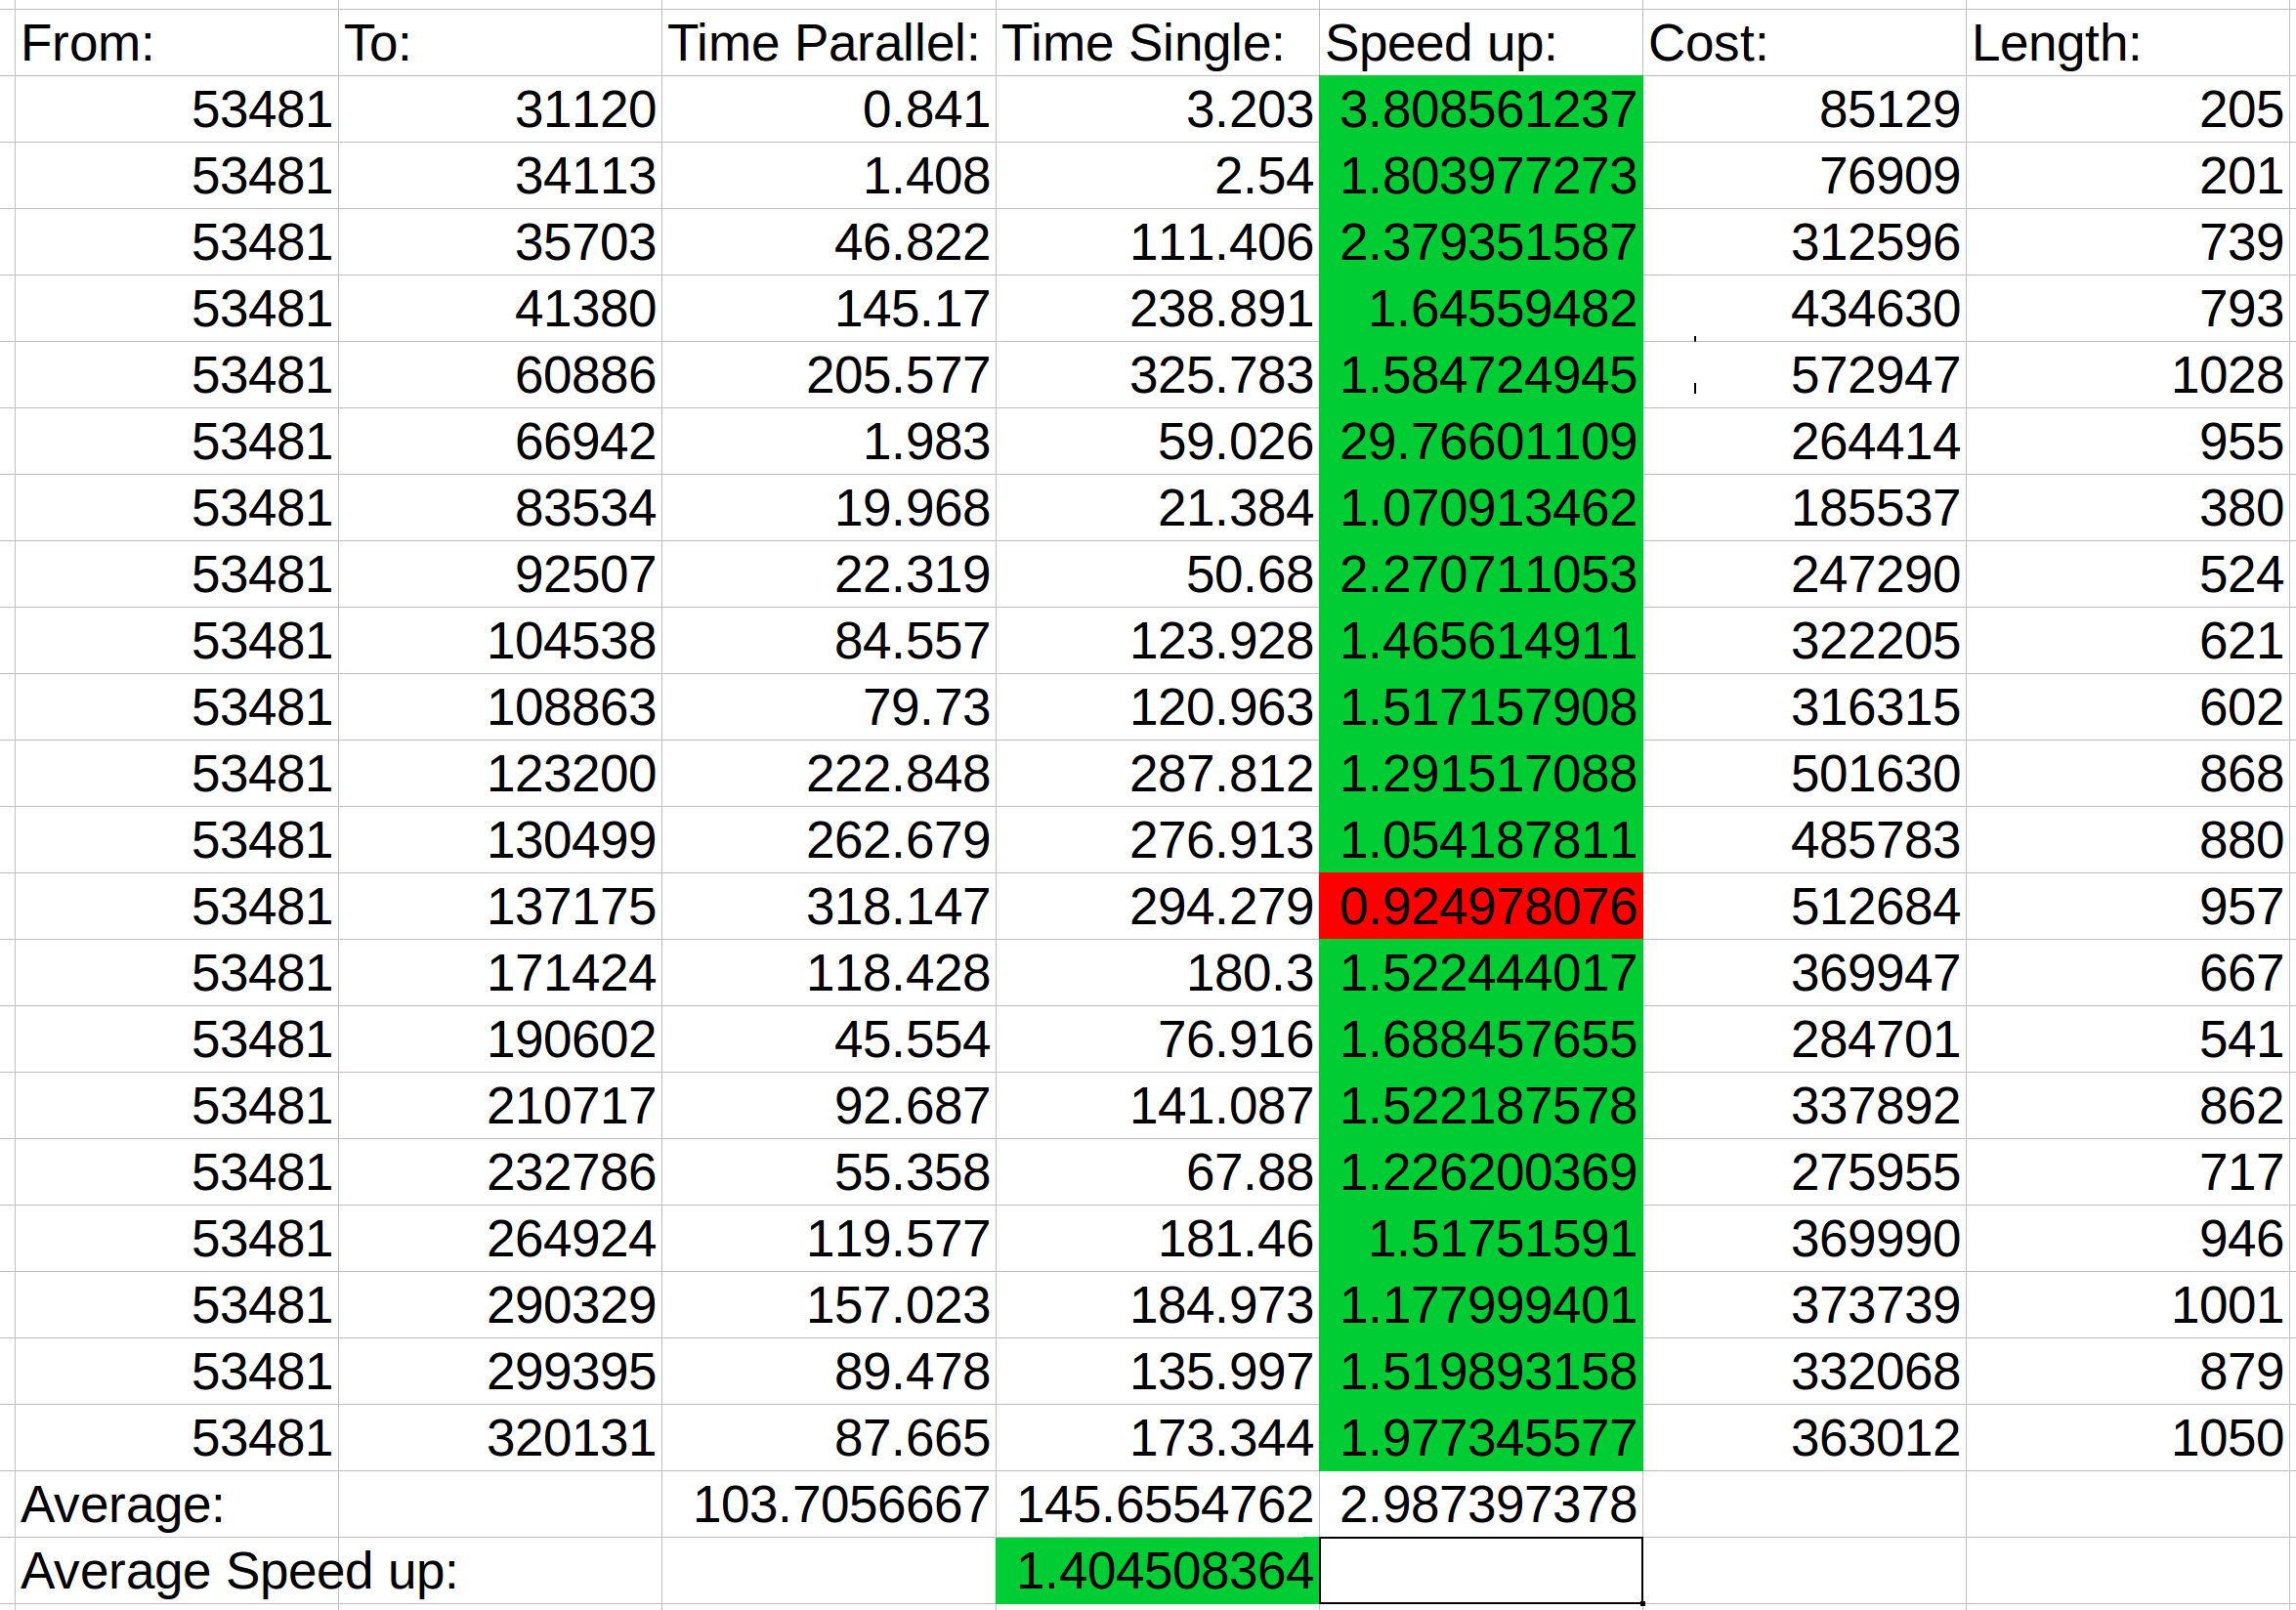
\includegraphics[scale=0.15]{summary1.png}

For my randomly generated graphs, I found the following:

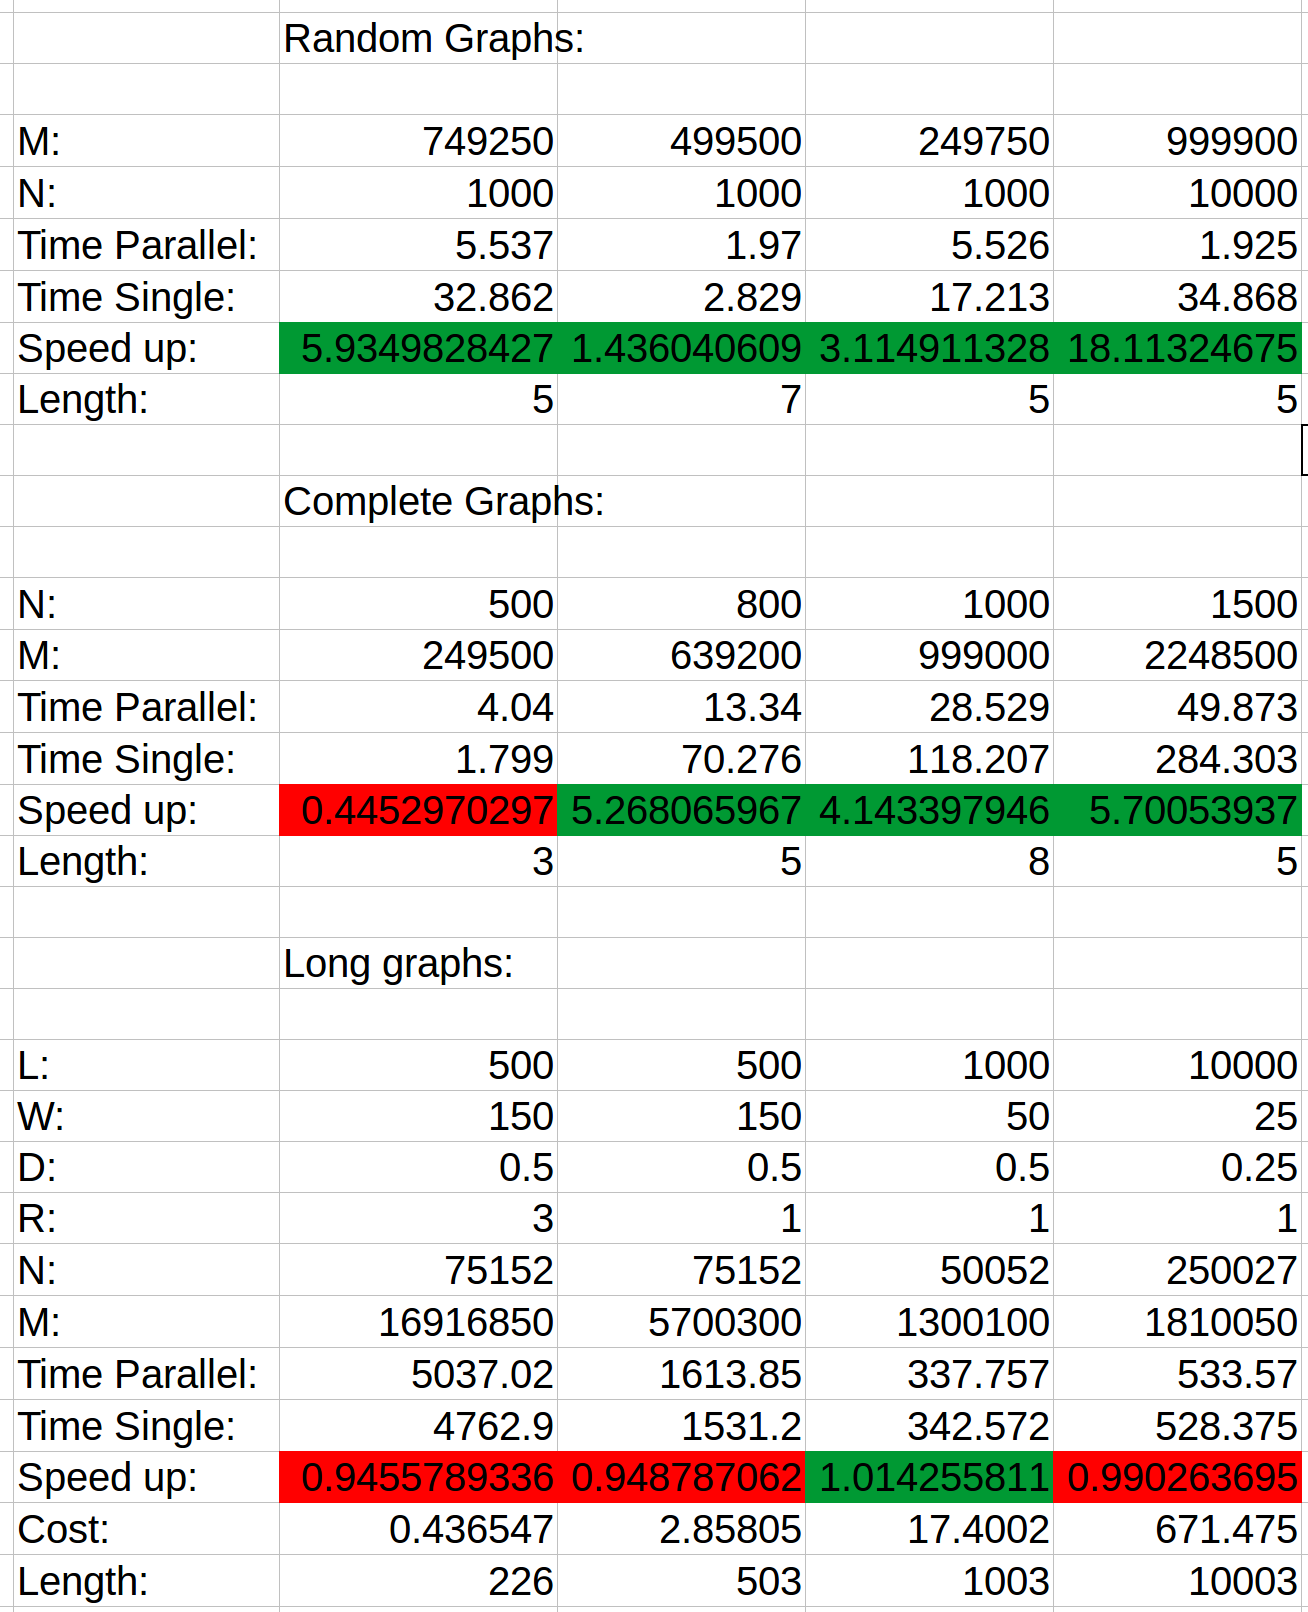
\includegraphics[scale=0.25]{summary2.png}

The results are interesting.
I had expected that on the long graphs, as the width $\to 1$ and the length $\to \infty$ that the speed up would approach $2$.
However, this is not what I found, and I am not sure why.

For the random graphs, it looks as though the larger the graph, the more of a speed up we see from parallel Dijkstra.
%However, there must be some optimal probability of adding an edge that make the speed up more.
It appears that the larger the graph, the more the speed up.
%,  am conjecturing this, because the speed increased 
I had conjectured that there would be an optimal probability of adding an edge to make the speed up the largest.
However, the probabilities went from .75 to .5 to .25 to .1, and on each instance, parallel Dijkstra's speed up increased.

For the complete graphs, there might be a tendency for the speed up to increase as $n\to\infty$.
However, I am not willing to conclude this yet, as going from 800 to 1000 vertices actually decreased the speed up.
These are all single runs though, and I cannot be sure how much variance there is between runs.
Anecdotally, I think there is not much between runs, although there may be differences between particular graphs with similar parameters.


\section{Concluding Remarks}


My code is on github at \cite{code}, although it has several hardcoded parameters.
If you were interested in using, I could move parameters to the command line and make it read your files without requiring you to run the python script.

We have seen that it is possible to parallelize Dijkstra's algorithm with a fairly simple modification of running two instances of Dijkstra's algorithm from both the source and sink node.
My implementation of this algorithm seems to be working well on a all four different types of graphs that I have tried it on: long graphs, random graphs, complete graphs and graphs from a real-world application.
In general, it appears that the speed up is greater for larger, more dense graphs.
This is not surprising.
One thing that is surprising is how much of a speed up is seen on some types of graphs.
This shows that parallelizing an algorithm can lead to a greater speed up than the number of processors.
However, even a single threaded algorithm could dove-tail a search from both nodes.
This means that much of the performance increase may come from the modification to the algorithm, rather than strictly the parallelization.

There are many more ways to improve this.
For example, different locking mechanisms could be explored, as well as an all pairs version that would scale with the number of processors by letting some threads start in the middle of the graph.
Also, this should be compared to parallel versions already implemented that simply parallelize the removal of nodes from the horizon.
These versions may have variability with respect to the data structure used within the heap: whether it be a binary heap (what this paper used), Fibonacci heap, or a Dial's implementation structure.
In addition to this, a single threaded application could be more efficient by not storing reverse edges.
The number of page faults may be significant with graphs as large as these.

Finally, it would be satisfying to have an explanation why parallel Dijkstra did not perform twice as fast as single Dijkstra on very long graphs.



\pagebreak


\begin{thebibliography}{9}
\bibitem{dijk}
\begin{verbatim}
https://web.engr.oregonstate.edu/~glencora/wiki/uploads/dijkstra-proof.pdf
\end{verbatim}

\bibitem{par1}
\begin{verbatim}
A. Crauser, K. Mehlhorn, U. Meyer, P. Sanders, ``A parallelization of Dijikstra’s
shortest path algorithm", in Proc. of MFCS’98, pp. 722-731, 1998.
\end{verbatim}


\bibitem{par2}
\begin{verbatim}
Y. Tang, Y. Zhang, H. Chen, ``A Parallel Shortest Path Algorithm Based on GraphPartitioning
and Iterative Correcting", in Proc. of IEEE HPCC’08, pp. 155-161,
2008.
\end{verbatim}

\bibitem{par3}
\begin{verbatim}
G. Stefano, A. Petricola, C. Zaroliagis, ``On the implementation of parallel shortest
path algorithms on a supercomputer", in Proc. of ISPA’06, pp. 406-417, 2006.
\end{verbatim}

\bibitem{code}
\begin{verbatim}
https://github.com/tlhallock/CodeForNetworkFlows
\end{verbatim}

\end{thebibliography}


\end{document}
